\begin{IEEEbiography}[{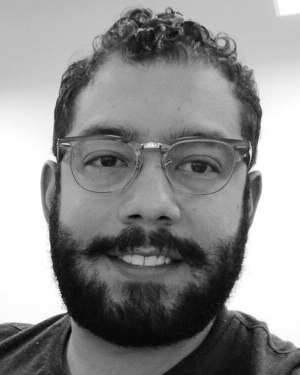
\includegraphics[width=1in,height=1.25in,clip,keepaspectratio]{../biography/yarib_300_375.jpg}}]{Yarib Nevarez} received the B.E. (Hons) degree in electronics from the Durango Institute of Technology, Durango, Mexico, in 2009, and the M.Sc. degree in Embedded Systems Design from the University of Applied Sciences Bremerhaven, Bremen, Germany, in 2017. He is currently pursuing a PhD degree with the Institute of Electrodynamics and Microelectronics, University of Bremen, Germany. His research interest is focused mainly on System-on-Chip architectures and hardware implementation for deep learning accelerators in Embedded Systems.
\\
During his professional experience, he served as a Senior Embedded Software Engineer at Texas Instruments, IBM, Continental Automotive, TOSHIBA, and Carbon Robotics. He has designed and developed software architectures for graphic calculators, automotive systems, robotic drivers, and more.
	
\end{IEEEbiography}

\begin{IEEEbiography}[{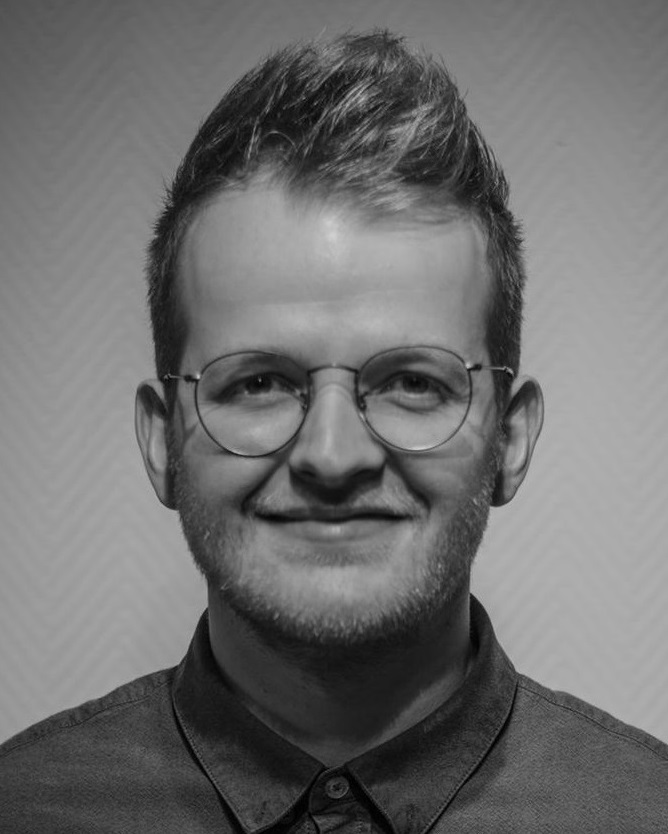
\includegraphics[width=1in,height=1.25in,clip,keepaspectratio]{../biography/Beering_bw_klein.jpeg}}]{Andreas Beering} received his B.Sc. and M.Sc. degree in Electrical and Information Engineering  from the University of Bremen, Germany, in 2015 and 2017, respectively. He is currently working towards a Ph.D. degree at the Institute of Electrodynamics and Microelectronics at the University of Bremen, Germany. His research interests focus mainly on signal processing and classification of vibration signals. In addition to the analysis of passive acoustic emission for monitoring gearboxes and processes, the second focus lies on active ultrasonic investigations.
In this context, ultrasonic waveforms for monitoring overmoulding processes are being investigated.
\end{IEEEbiography}

\begin{IEEEbiography}[{
\includegraphics[width=1in,height=1.25in,clip,keepaspectratio]{../biography/person.png}}]{Amir Najafi}
\end{IEEEbiography}

\begin{IEEEbiography}[{
\includegraphics[width=1in,height=1.25in,clip,keepaspectratio]{../biography/person.png}}]{Ardalan Najafi}
\end{IEEEbiography}

\begin{IEEEbiography}[{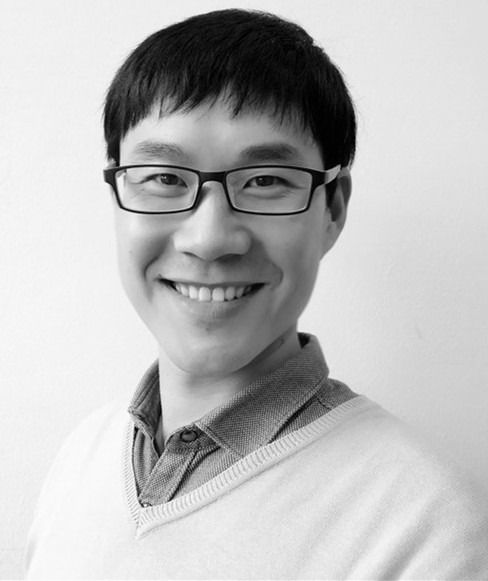
\includegraphics[width=1in,height=1.25in,clip,keepaspectratio]{../biography/wyu.jpg}}]{Wanli Yu}
	
	received the B. S. degree in information engineering and the M. S. degree in signal and information processing from the China University of Mining and Technology, Xuzhou, China, in 2009 and 2012, respectively and the PhD degree from the University of Bremen, Germany, in 2018.
	
	He is currently a Post-Doctoral Researcher with the Institute of Electrodynamics and Microelectronics, University of Bremen. His research interests include sensor networks, Internet of Things, network performance optimization, energy aware task allocation and scheduling, mobile edge/fog computing, convex optimization, machine learningand nature-inspired population-based optimization.
\end{IEEEbiography}

\begin{IEEEbiography}[{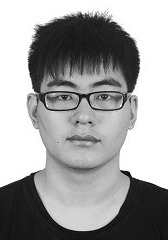
\includegraphics[width=1in,height=1.25in,clip,keepaspectratio]{../biography/YizhiChen.jpg}}]{Yizhi Chen} received the B.E. degree in Electronic and Information Engineering from Wuhan University, China, in 2017 and he received the M.S. degree in Communication and Information Technology from the University of Bremen, Germany, in 2021. Currently, he is working as a Ph.D. student at the Division of Electronics and Embedded Systems, Department of Electrical Engineering, School of Electrical Engineering and Computer Science, KTH Royal Institute of Technology, Sweden. His research interests include hardware accelerator for ML, fault-tolerant hardware for neural networks, Network-on-Chip, and approximate computing.
\end{IEEEbiography}

\begin{IEEEbiography}[{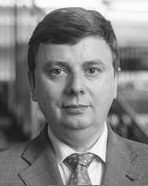
\includegraphics[width=1in,height=1.25in,clip,keepaspectratio]{../biography/krieger.jpg}}]{Karl-Ludwig Krieger} received his Ph.D. degree in Electrical Engineering in 1999 from the University of Bremen, Germany. Dr. Krieger worked from 1998-2009 as a manager in the field of function and algorithm development for powertrain systems at Daimler AG in Stuttgart. Since 2009 he has been a full professor for the chair of Electronic Vehicle and Mobility Systems at the University of Bremen, Germany. The research focus of his chair is primarily on the analysis of vibration and ultrasound signals in different application fields, for example, passenger cars, heavy-duty trucks, mobile working machines or industrial machines. Further research priorities of the chair are near-infrared spectral sensors and capacitive sensor systems for different fields of application. These research topics are worked on in close cooperation with leading industrial partners and are mainly financed from third-party funds.
\end{IEEEbiography}

\begin{IEEEbiography}[{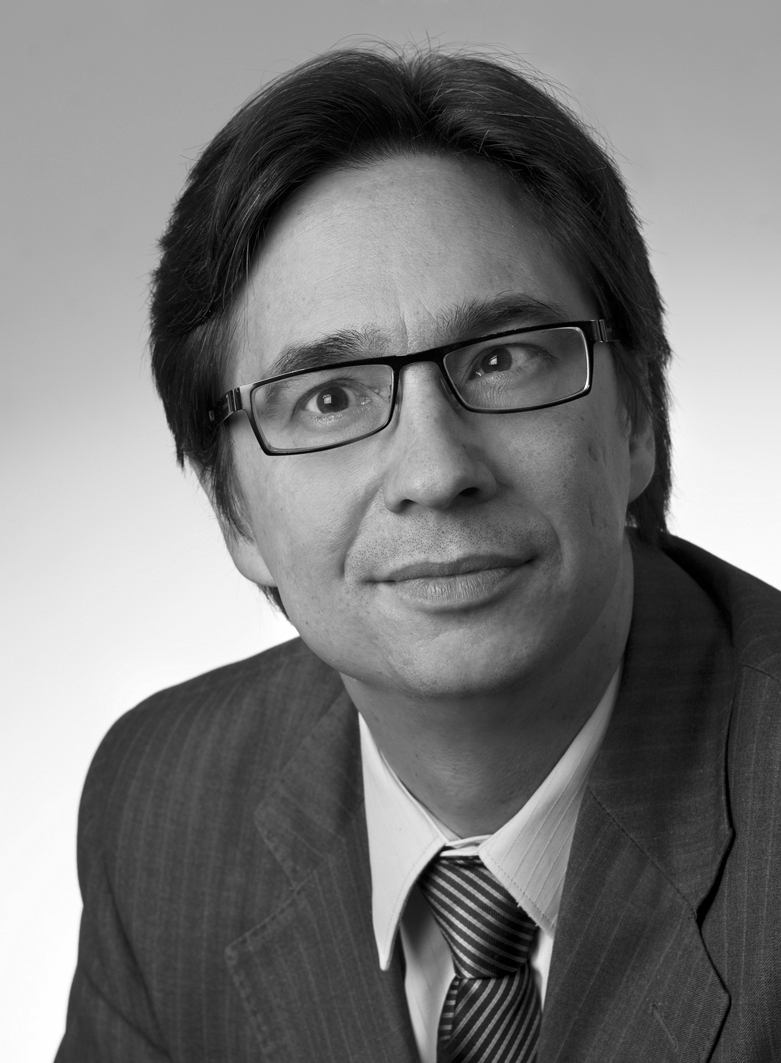
\includegraphics[width=1in,height=1.25in,clip,keepaspectratio]{../biography/Alberto_Garcia-Ortiz.jpg}}]{Alberto Garcia-Ortiz}
    obtained the diploma degree in
    Telecommunication Systems from the Polytechnic University of
    Valencia (Spain) in 1998. After working for two years at Newlogic
    in Austria, he started the Ph.D. at the Institute of
    Microelectronic Systems, Darmstadt University of Technology,
    Germany. In 2003, he received from the Department of Electrical
    Engineering and Information Technology of the university the
    Ph.D. degree with "summa cum laude." From 2003 to 2005, he worked
    as a Senior Hardware Design Engineer at IBM Deutschland
    Development and Research in B{\"o}blingen.  After that he joined the
    start-up AnaFocus (Spain), where he was responsible for the design
    and integration of AnaFocus" next generation Vision
    Systems-on-Chip. He is currently full professor for the chair of
    integrated digital systems at the university of Bremen.
    Dr. Garcia-Ortiz received the "Outstanding dissertation award" in
    2004 from the European Design and Automation Association. In 2005,
    he received from IBM an innovation award for contributions to
    leakage estimation. Two patents are issued with that work. He
    serves as editor of JOLPE and is reviewer of several conferences,
    journals, and European projects. \\
    His interests include low-power
    design and estimation, communication- centric design, SoC
    integration, and variations-aware design. 
\end{IEEEbiography}
